\subsection{High order correction for $dE$}
\begin{figure}[htbp]
  \begin{tabular}{cc}
    \begin{minipage}{0.5\hsize}
      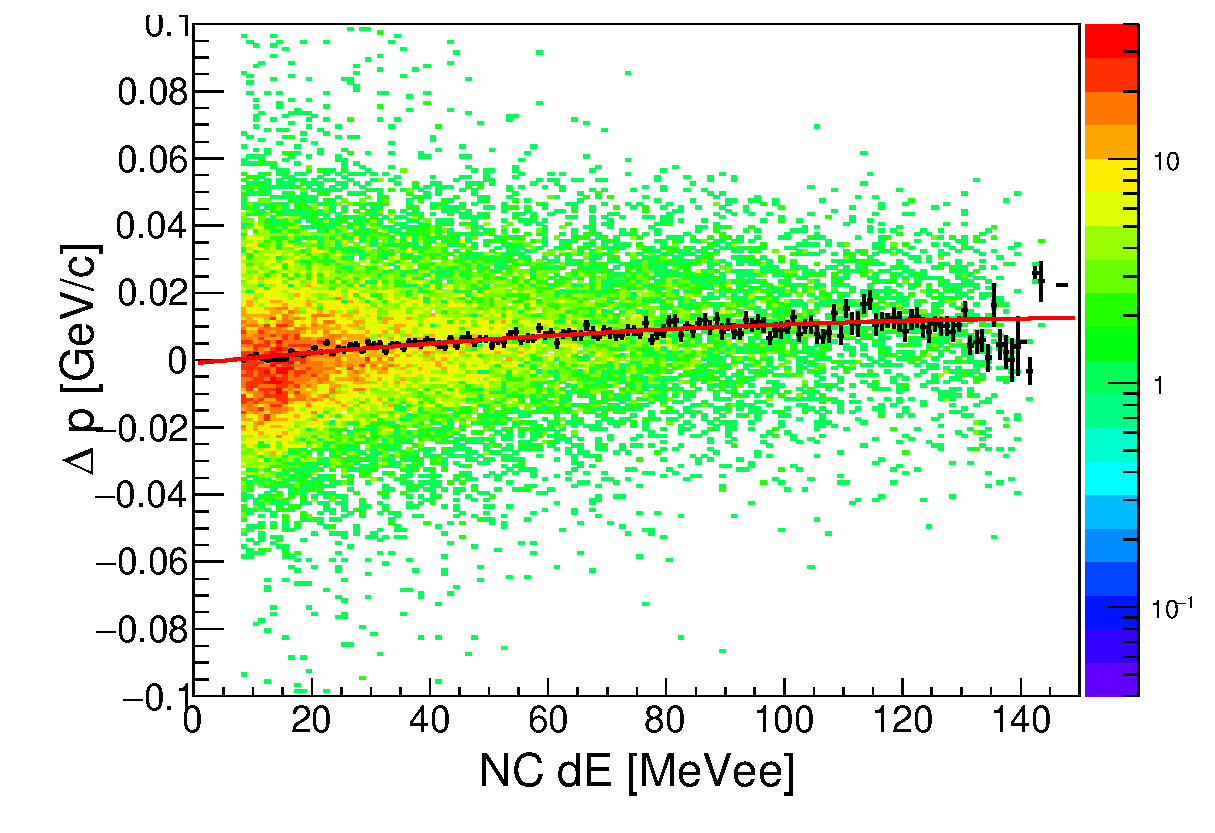
\includegraphics[width=5cm]{../pic/Run78/calib/NCdE_delta_p.eps}
    \end{minipage}
    \begin{minipage}{0.5\hsize}
      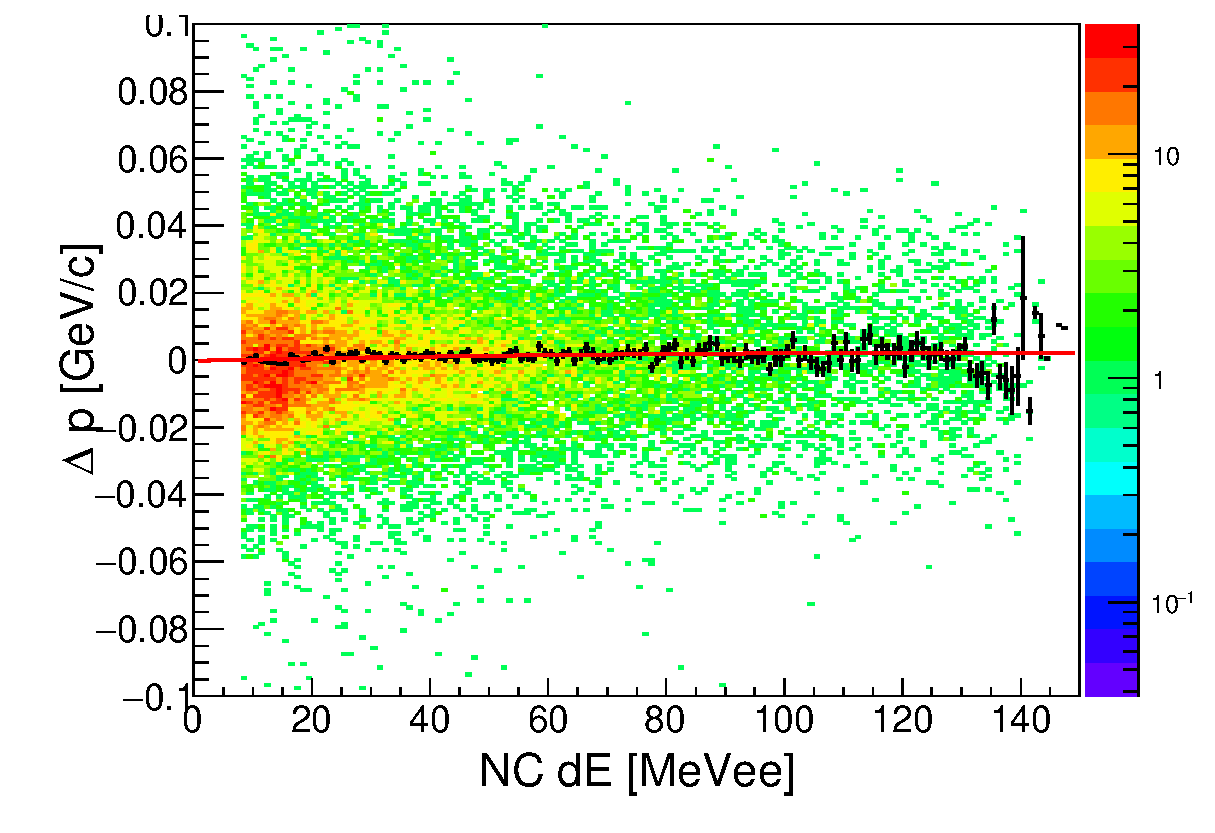
\includegraphics[width=5cm]{../pic/Run78/calib/NCdE_delta_p_mod.eps}
    \end{minipage}
  \end{tabular}
  \caption{
    These figures show $\Delta$ p which was calculated by given PDG value of neutron mass.
    Left figure represents before calibration and right figure represents after calibration.
  }
  \label{fig:NC_recalib}
\end{figure}

%% todo %% 英語の直し
The NC time walk effect was calibrated by $\gamma$ conversion events around the target system which was seen in Fig\ref{fig:NC_beta}.
So neutron made large energe deposit events,
$\gamma$ events was not enough for calibration of large energy deposit correction which was seen in $d(K^-, n \pi^+ \pi^-)"n"$ events that is described after section.
Fig\ref{fig:NC_recalib} shows these effect which was convert to time offset giving true PDG value of neutron.
This effect was calibrated using 3rd polynomial function which is shown in same figure.


